\documentclass[10pt,a4paper]{article}
\usepackage[utf8]{inputenc}
\usepackage[spanish]{babel}
\usepackage{amsmath}
\usepackage{amsfonts}
\usepackage{amssymb}
\usepackage{enumitem}
\usepackage{hyperref} 
\usepackage{graphicx}
\usepackage[margin=0.5in]{geometry}
\hypersetup{pdftex,colorlinks=true,allcolors=blue}
\hypersetup{
    pdftitle={},
    pdfauthor={Pablo Riutort Grande},
    pdfsubject={},
    bookmarksnumbered=true,     
    bookmarksopen=true,         
    bookmarksopenlevel=1,       
    colorlinks=true,            
    pdfstartview=Fit,           
    pdfpagemode=UseOutlines,    % this is the option you were lookin for
    pdfpagelayout=TwoPageRight
}
\usepackage{listings}
\usepackage{xcolor}
\usepackage{hypcap}
\definecolor{codegreen}{rgb}{0,0.6,0}
\definecolor{codegray}{rgb}{0.5,0.5,0.5}
\definecolor{codepurple}{rgb}{0.58,0,0.82}
\definecolor{backcolour}{rgb}{0.95,0.95,0.92}
\lstdefinestyle{mystyle}{
    backgroundcolor=\color{backcolour},   
    commentstyle=\color{codegreen},
    keywordstyle=\color{magenta},
    numberstyle=\tiny\color{codegray},
    stringstyle=\color{codepurple},
    basicstyle=\ttfamily\footnotesize,
    breakatwhitespace=false,         
    breaklines=true,                 
    captionpos=b,                    
    keepspaces=true,                 
    numbers=left,                    
    numbersep=5pt,                  
    showspaces=false,                
    showstringspaces=false,
    showtabs=false,                  
    tabsize=2
}
\lstset{style=mystyle}
\usepackage{xparse}
\NewDocumentCommand{\codeword}{v}{%
\texttt{{#1}}
}
\author{Pablo Riutort Grande}
\title{Seguridad en Sistemas Operativos \\\vspace{0.3cm}PEC 2\\ \vspace{1cm}\textbf{Securizar servidores, análisis de puertos}}

\begin{document}
\maketitle

\section{Linux Server}
Para este apartado se ha instalado y configurado software que utiliza algunos puertos de la máquina virtual:
\begin{itemize}
\item nginx: Para los puertos 22, 80 y 443
\item CUPS: Utiliza el puerto 631
\item FTP: Utiliza el puerto 21
\end{itemize}

\begin{lstlisting}[language=bash]
apt update -y; apt install -y nginx openssh-server cups vsftpd ftp
\end{lstlisting}
Generamos un certificado autofirmado y configuramos nginx para que lo utilice \cite{nginx}, de esta forma podemos servir mediante nginx conexiones a través del puerto 443 (SSL).

\begin{enumerate}[label=\textbf{\alph*)}]
\item nmap:
\begin{lstlisting}[language=bash]
root@debian:~# nmap -sV localhost
Starting Nmap 7.70 ( https://nmap.org ) at 2020-04-05 22:23 CEST
Nmap scan report for localhost (127.0.0.1)
Host is up (0.000012s latency).
Other addresses for localhost (not scanned): ::1
Not shown: 995 closed ports
PORT    STATE SERVICE  VERSION
21/tcp  open  ftp      vsftpd 3.0.3
22/tcp  open  ssh      OpenSSH 7.9p1 Debian 10+deb10u2 (protocol 2.0)
80/tcp  open  http     nginx 1.14.2
443/tcp open  ssl/http nginx 1.14.2
631/tcp open  ipp      CUPS 2.2
Service Info: OSs: Unix, Linux; CPE: cpe:/o:linux:linux_kernel

Service detection performed. Please report any incorrect results at https://nmap.org/submit/ .
Nmap done: 1 IP address (1 host up) scanned in 14.17 seconds
\end{lstlisting}
netstat:
\begin{lstlisting}[language=bash]
root@debian:~# netstat --listening
Active Internet connections (only servers)
Proto Recv-Q Send-Q Local Address           Foreign Address         State      
tcp        0      0 0.0.0.0:http            0.0.0.0:*               LISTEN     
tcp        0      0 0.0.0.0:ssh             0.0.0.0:*               LISTEN     
tcp        0      0 localhost:ipp           0.0.0.0:*               LISTEN     
tcp        0      0 0.0.0.0:https           0.0.0.0:*               LISTEN     
tcp6       0      0 [::]:http               [::]:*                  LISTEN     
tcp6       0      0 [::]:ftp                [::]:*                  LISTEN     
tcp6       0      0 [::]:ssh                [::]:*                  LISTEN     
tcp6       0      0 localhost:ipp           [::]:*                  LISTEN     
tcp6       0      0 [::]:https              [::]:*                  LISTEN     
udp        0      0 0.0.0.0:ipp             0.0.0.0:*                          
udp        0      0 0.0.0.0:mdns            0.0.0.0:*                          
udp        0      0 0.0.0.0:46806           0.0.0.0:*                          
udp        0      0 0.0.0.0:bootpc          0.0.0.0:*                          
udp6       0      0 [::]:mdns               [::]:*                             
udp6       0      0 [::]:47332              [::]:*                             
raw6       0      0 [::]:ipv6-icmp          [::]:*                  7          
Active UNIX domain sockets (only servers)
Proto RefCnt Flags       Type       State         I-Node   Path
unix  2      [ ACC ]     STREAM     LISTENING     19784    /tmp/.ICE-unix/721
unix  2      [ ACC ]     STREAM     LISTENING     10499    /run/systemd/journal/stdout
unix  2      [ ACC ]     STREAM     LISTENING     17770    /tmp/.X11-unix/X0
unix  2      [ ACC ]     STREAM     LISTENING     19628    /tmp/ssh-kx6ERuyTOjOS/agent.680
unix  2      [ ACC ]     STREAM     LISTENING     17769    @/tmp/.X11-unix/X0
unix  2      [ ACC ]     SEQPACKET  LISTENING     10786    /run/udev/control
unix  2      [ ACC ]     STREAM     LISTENING     19783    @/tmp/.ICE-unix/721
unix  2      [ ACC ]     STREAM     LISTENING     17485    /run/NetworkManager/private-dhcp
unix  2      [ ACC ]     STREAM     LISTENING     14216    /var/run/dbus/system_bus_socket
unix  2      [ ACC ]     STREAM     LISTENING     14221    /run/cups/cups.sock
unix  2      [ ACC ]     STREAM     LISTENING     14225    /run/avahi-daemon/socket
unix  2      [ ACC ]     STREAM     LISTENING     19727    @/tmp/dbus-cLiJoZjMM2
unix  2      [ ACC ]     STREAM     LISTENING     19429    /run/user/0/systemd/private
unix  2      [ ACC ]     STREAM     LISTENING     19436    /run/user/0/gnupg/S.gpg-agent.browser
unix  2      [ ACC ]     STREAM     LISTENING     19439    /run/user/0/gnupg/S.dirmngr
unix  2      [ ACC ]     STREAM     LISTENING     10479    /run/systemd/private
unix  2      [ ACC ]     STREAM     LISTENING     19441    /run/user/0/gnupg/S.gpg-agent.ssh
unix  2      [ ACC ]     STREAM     LISTENING     19443    /run/user/0/gnupg/S.gpg-agent.extra
unix  2      [ ACC ]     STREAM     LISTENING     19445    /run/user/0/gnupg/S.gpg-agent
unix  2      [ ACC ]     STREAM     LISTENING     19447    /run/user/0/bus
unix  2      [ ACC ]     STREAM     LISTENING     10488    /run/systemd/fsck.progress
\end{lstlisting}

\item Los servicios que utilizan puertos que no son 22, 80 y 443 son ftp (21) y CUPS (631). Para deshabilitar estos procesos ejecutamos los comandos systemctl stop y disable:
\begin{lstlisting}[language=bash]
root@debian:~# systemctl stop vsftpd
root@debian:~# systemctl disable vsftpd
Synchronizing state of vsftpd.service with SysV service script with /lib/systemd/systemd-sysv-install.
Executing: /lib/systemd/systemd-sysv-install disable vsftpd
Removed /etc/systemd/system/multi-user.target.wants/vsftpd.service.
root@debian:~# systemctl stop cups
root@debian:~# systemctl disable cups
Synchronizing state of cups.service with SysV service script with /lib/systemd/systemd-sysv-install.
Executing: /lib/systemd/systemd-sysv-install disable cups
Removed /etc/systemd/system/printer.target.wants/cups.service.
Removed /etc/systemd/system/multi-user.target.wants/cups.path.
Removed /etc/systemd/system/sockets.target.wants/cups.socket.
root@debian:~# systemctl stop cups-browsed
root@debian:~# systemctl disable cups-browsed
Synchronizing state of cups-browsed.service with SysV service script with /lib/systemd/systemd-sysv-install.
Executing: /lib/systemd/systemd-sysv-install disable cups-browsed
Removed /etc/systemd/system/multi-user.target.wants/cups-browsed.service.
\end{lstlisting}

En el caso de que quisiéramos actualizar los enlaces a los scripts de init para prevenir la ejecución al cambiar el nivel de ejecución podemos ejecutar \cite{update-rc}:
\begin{lstlisting}[language=bash]
root@debian:~# update-rc.d vsftpd remove
root@debian:~# update-rc.d cups remove
\end{lstlisting}

Después de parar y deshabilitar los servicios relativos a ftp y CUPS reiniciamos. Al ejecutar nuevamente el comando nmap sobre localhost vemos que los únicos servicios en funcionamiento son los relativos a los puertos 22, 80 y 443.

\begin{lstlisting}[language=bash]
root@debian:~# nmap -sV localhost
Starting Nmap 7.70 ( https://nmap.org ) at 2020-04-07 01:00 CEST
Nmap scan report for localhost (127.0.0.1)
Host is up (0.000021s latency).
Other addresses for localhost (not scanned): ::1
Not shown: 997 closed ports
PORT    STATE SERVICE  VERSION
22/tcp  open  ssh      OpenSSH 7.9p1 Debian 10+deb10u2 (protocol 2.0)
80/tcp  open  http     nginx 1.14.2
443/tcp open  ssl/http nginx 1.14.2
Service Info: OS: Linux; CPE: cpe:/o:linux:linux_kernel

Service detection performed. Please report any incorrect results at https://nmap.org/submit/ .
Nmap done: 1 IP address (1 host up) scanned in 14.17 seconds
\end{lstlisting}

\item Primera prueba de ping desde host:
\begin{lstlisting}[language=bash]
~ $ ping 192.168.1.172
PING 192.168.1.172 (192.168.1.172) 56(84) bytes of data.
64 bytes from 192.168.1.172: icmp_seq=1 ttl=64 time=0.947 ms
64 bytes from 192.168.1.172: icmp_seq=2 ttl=64 time=0.559 ms
64 bytes from 192.168.1.172: icmp_seq=3 ttl=64 time=0.580 ms
^C
--- 192.168.1.172 ping statistics ---
3 packets transmitted, 3 received, 0% packet loss, time 2015ms
rtt min/avg/max/mdev = 0.559/0.695/0.947/0.179 ms
\end{lstlisting}
Las máquinas pueden verse y hay respuesta con ping. Ahora deshabilitamos el ping de la máquina virtual con los comandos: \cite{ping}
\begin{lstlisting}[language=bash]
echo 1 > /proc/sys/net/ipv4/icmp_echo_ignore_all
echo  "net.ipv4.icmp_echo_ignore_all = 1" >> /etc/sysctl.conf
sysctl -p
\end{lstlisting}
Reiniciamos la máquina, realizamos nuevamente el ping y vemos que no recibimos ningún paquete de vuelta:
\begin{lstlisting}[language=bash]
~ $ ping 192.168.1.172
PING 192.168.1.172 (192.168.1.172) 56(84) bytes of data.
^C
--- 192.168.1.172 ping statistics ---
3 packets transmitted, 0 received, 100% packet loss, time 2051ms
\end{lstlisting}

\item A continuación se muestra el proceso por el cual logramos una Shell desde el Grub: \cite{boot}

\begin{figure}[h!]
  \centering
  
\includegraphics[scale=0.6]{d1.png}\\
  \caption{Entramos a través del grub en \textit{recovery mode}}
  \label{fig:grub1}
\end{figure}
\begin{figure}[h!]
  \centering
  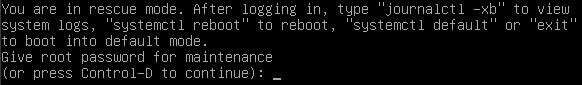
\includegraphics[scale=0.6]{d2.png}\\
  \caption{Introducimos la contraseña de \textit{root}}
  \label{fig:grub2}
\end{figure}
\begin{figure}[h!]
  \centering
  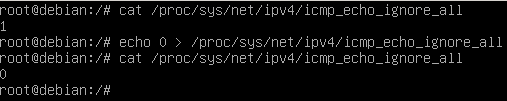
\includegraphics[scale=0.6]{d3.png}\\
  \caption{Tenemos una shell en modo root. Efecutamos algunos cambios}
  \label{fig:grub3}
\end{figure}
\begin{figure}[h!]
  \centering
  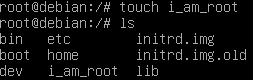
\includegraphics[scale=0.6]{i_am_root.png}\\
  \caption{Creamos archivos en la raíz}
  \label{fig:grub4}
\end{figure}
\begin{figure}[h!]
  \centering
  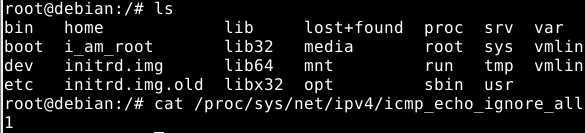
\includegraphics[scale=0.6]{d4.png}\\
  \caption{Una vez dentro del sistema vemos que los cambios son persistentes}
  \label{fig:grub5}
\end{figure}
\item 
\pagebreak
\begin{enumerate}[label=\arabic*.]
\item Generamos una password segura con el comando \textbf{grub-mkpasswd-pbkdf2}
\item Añadimos al archivo \textbf{/etc/grub.d/00\_header}:
\begin{lstlisting}[language=bash]
cat << EOF
set superusers="root"
password_pbkdf2 root <password generado en paso anterior>
EOF
\end{lstlisting}
\item Ejecutamos el comando \textbf{update-grub2}
\item Reiniciamos

\end{enumerate}

\end{enumerate}

\begin{figure}[h!]
  \centering
  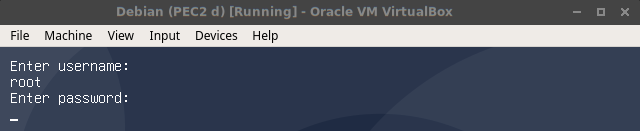
\includegraphics[scale=0.6]{e.png}\\
  \caption{Grub protegido por usuario y contraseña \cite{grub}}
  \label{fig:grub}
\end{figure}

\section{Windows Server}
\begin{enumerate}[label=\textbf{\alph*)}]
\setcounter{enumi}{5}
\item %f
Microsoft Compliance Toolkit es un conjunto de herramientas que permite a un administrador gestionar los objetos de políticas de grupo (\textit{Group Policy Objects} o \textit{GPO}). Mediante esta herramienta se pueden comparar estos objetos con los recomendados por Microsoft u otras bases de políticas; se pueden editar, guardar y aplicar a través del Active Directory o individualmente \cite{SCT}.
\\
\begin{figure}[h!]
  \centering
  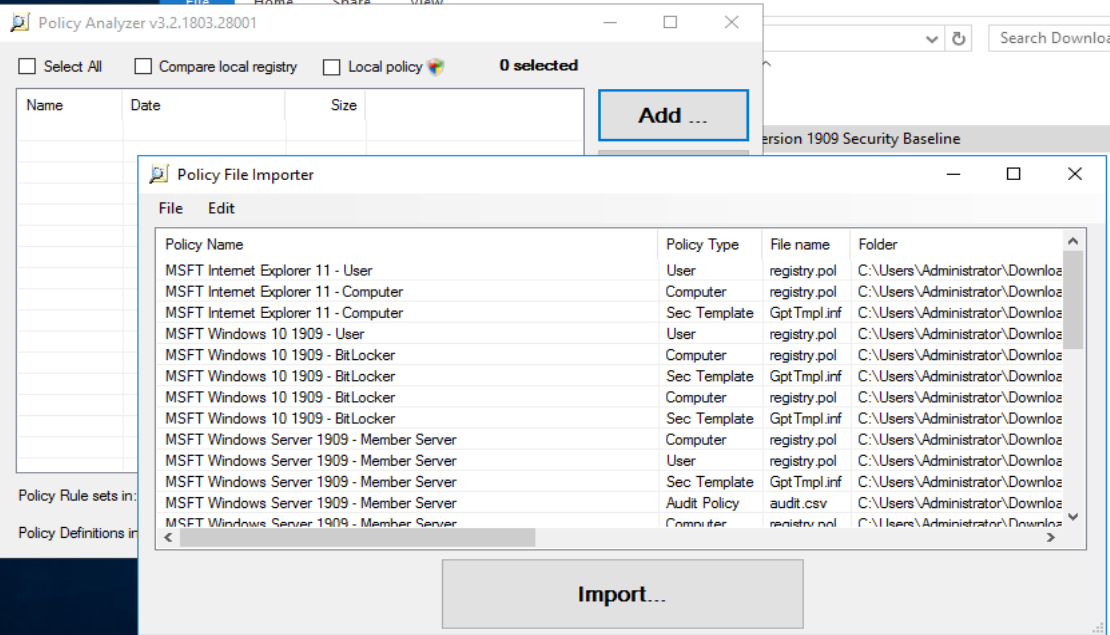
\includegraphics[scale=0.2]{f.png}\\
  \caption{Para importar las GPOs ejecutamos el programa de PolicyAnalyzer y añadimos las políticas que se encuentran en ``Windows 10 Version 1909 and Windows ServerVersion 1909 Security Baseline/GPOs''}
  \label{fig:gpos}
\end{figure}

Para hacer una copia de seguridad de las políticas locales ejecutamos la herramienta de Group Policy Management Console con el comando gpmc.msc, seleccionamos Forest: uoc.local $>$ Domains $>$ View $>$ Options $>$ Table location: Group Policy Objects.\\
Seleccionamos el dominio uoc.local $>$ Group Policy Objects y con click derecho tendremos la opción de Back Up All\ldots y seleccionamos un directorio donde guardar los GPOs \cite{gpo_backup}. Finalmente, ejecutamos la herramienta Policy Analyzer nuevamente para importarlas.\\
La herramienta de Policy Analyzer nos permite comparar las GPOs de Baseline con las importadas del entorno local y existen una serie de configuraciones \textbf{conflictivas}:
\begin{itemize}
\item \textit{Credential Validation}: Permite revisar eventos generados por validación de credenciales. No especificado en la política local.
\item \textit{LsaCfgFlags}: Especifica si la seguridad basada en virtualización está habilitada. No especificada en local.
\item \textit{SeDenyNetworkLogonRight}: Deniega el acceso al ordenador desde la red. No especificada en local.
\item \textit{SeEnableDelegationPrivilege}: Permite a las cuentas de usuario confiables para la delegación.
\item \textit{SeInteractiveLogonRight}: Permite el login de manera local. Existen discrepancias entre los flags de la política de baseline y los de la local.
\item \textit{SeNetworkLogonRight}: Permite el acceso al ordenador desde la red. Los flags de baseline son distintos a los de la política local.
\end{itemize}

\item %g
\begin{lstlisting}
PS C:\Users\Administrator> netstat -ab -p TCP

Active Connections

  Proto  Local Address          Foreign Address        State
  TCP    0.0.0.0:80             UOC1:0                 LISTENING
 Can not obtain ownership information
  TCP    0.0.0.0:88             UOC1:0                 LISTENING
 [lsass.exe]
  TCP    0.0.0.0:135            UOC1:0                 LISTENING
  RpcSs
 [svchost.exe]
  TCP    0.0.0.0:389            UOC1:0                 LISTENING
 [lsass.exe]
  TCP    0.0.0.0:445            UOC1:0                 LISTENING
 Can not obtain ownership information
  TCP    0.0.0.0:464            UOC1:0                 LISTENING
 [lsass.exe]
  TCP    0.0.0.0:593            UOC1:0                 LISTENING
  RpcEptMapper
 [svchost.exe]
  TCP    0.0.0.0:636            UOC1:0                 LISTENING
 [lsass.exe]
  TCP    0.0.0.0:3268           UOC1:0                 LISTENING
 [lsass.exe]
  TCP    0.0.0.0:3269           UOC1:0                 LISTENING
 [lsass.exe]
  TCP    0.0.0.0:5985           UOC1:0                 LISTENING
 Can not obtain ownership information
  TCP    0.0.0.0:9389           UOC1:0                 LISTENING
 [Microsoft.ActiveDirectory.WebServices.exe]
  TCP    0.0.0.0:47001          UOC1:0                 LISTENING
 Can not obtain ownership information
  TCP    0.0.0.0:49664          UOC1:0                 LISTENING
 Can not obtain ownership information
  TCP    0.0.0.0:49665          UOC1:0                 LISTENING
  EventLog
 [svchost.exe]
  TCP    0.0.0.0:49666          UOC1:0                 LISTENING
  Schedule
 [svchost.exe]
  TCP    0.0.0.0:49667          UOC1:0                 LISTENING
 [lsass.exe]
  TCP    0.0.0.0:49669          UOC1:0                 LISTENING
 [lsass.exe]
  TCP    0.0.0.0:49670          UOC1:0                 LISTENING
 [lsass.exe]
  TCP    0.0.0.0:49672          UOC1:0                 LISTENING
 [spoolsv.exe]
  TCP    0.0.0.0:49675          UOC1:0                 LISTENING
 Can not obtain ownership information
  TCP    0.0.0.0:49686          UOC1:0                 LISTENING
 [dns.exe]
  TCP    0.0.0.0:58996          UOC1:0                 LISTENING
 [DFSRs.exe]
  TCP    127.0.0.1:53           UOC1:0                 LISTENING
 [dns.exe]
  TCP    192.168.1.174:53       UOC1:0                 LISTENING
 [dns.exe]
  TCP    192.168.1.174:139      UOC1:0                 LISTENING
 Can not obtain ownership information
  TCP    192.168.1.174:58975    40.67.254.36:https     ESTABLISHED
 [Explorer.EXE]
  TCP    192.168.1.174:58981    51.124.78.146:https    TIME_WAIT
  TCP    192.168.1.174:58982    40.67.254.36:https     ESTABLISHED
  ProfSvc
 [svchost.exe]
  TCP    192.168.1.174:58983    51.124.78.146:https    TIME_WAIT
  TCP    192.168.1.174:58985    40.77.226.250:https    TIME_WAIT
  TCP    192.168.1.174:58987    51.124.78.146:https    ESTABLISHED
  UsoSvc
 [svchost.exe]
  TCP    192.168.1.174:58988    40.77.226.250:https    TIME_WAIT
  TCP    192.168.1.174:58989    13.74.179.117:https    TIME_WAIT
  TCP    192.168.1.174:59001    20.36.218.70:https     ESTABLISHED
  wuauserv
 [svchost.exe]
\end{lstlisting}
Todos los servicios listados son, en cierta medida, necesarios para el correcto funcionamiento del sistema. Quizá los procesos Explorer.EXE y DSFRs.exe son los mñas prescindibles en nuestro contexto puesto que el primero se trata del Explorador de archivos de Windows y el segundo permite la sincronización de ficheros entre múltiples servidores de la red local o WAN.\\
El proceso que utiliza el TCP/88 es el lsass.exe, es el proceso de autenticación de seguridad local de Microsoft, autentica la identificación de un usuario y la aplicación de políticas de seguridad. Al intentar matar el proceso la máquina se reinicia automáticamente así que, en principio, no parece que se pueda desactivar.

\item %h
Nmap funciona conectándose a cada puerto e intenta obtener información del tipo de servicio que está tras el puerto. Debido a su funcionamiento se trata de un proceso más lento y no puede mostrar el ID del proceso que se encuentra usando el puerto ya que se encuentra al otro lado de la máquina.\\
Netstat obtiene la información del Sistema Operativo a través del kernel. Puede sacar un listado de puertos que están en uso y obtener también el ID del proceso que lo está usando.\\

Tiene sentido usar nmap cuando se desea saber información de un sistema remoto, de los puertos que tenga abiertos y de los servicios escuchando en cada puerto. Se puede optar por usar netstat cuando se quiere saber qué proceso está usando cada puerto en la máquina local e incluso estadísticas de conexiones de red \cite{nmap-netstat}.

\begin{figure}[h!]
  \centering
  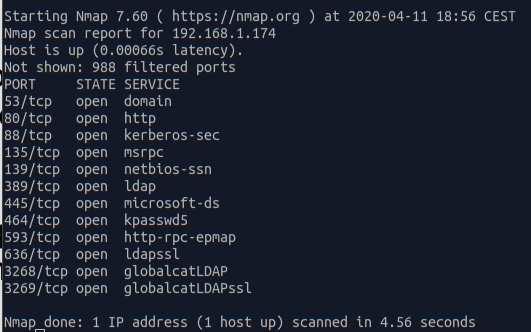
\includegraphics[scale=0.4]{h.png}\\
  \caption{Nmap desde Linux para ver los puertos en escucha en el equipo de Windows}
  \label{fig:nmap}
\end{figure}

\item %i
Para instalar un servidor web con estas características primero debemos crear un certificado que nos permita utilizar HTTPS \cite{https-win}.
\begin{enumerate}[label=\arabic*.]
\item Ejecutamos la aplicación de Internet Information Services (ISS) Manager.
\item Seleccionamos nuestro servidor UOC1 y Server Certificates bajo el área de ISS.
\item Aparecerá la opción de crear un certificado en el panel derecho. Lo seleccionamos.
\item Aparecerá una nueva ventana donde debemos asignar un nombre a nuestro certificado y un sitio donde guardarlo (Personal, Web Hosting).
\item Volvemos al panel izquierdo y seleccionamos UOC1 $>$ Sites $>$ Default Web Site y en el área derecha de la ventana nos aparecerá la opción de Bindings. La seleccionamos.
\item Añadimos un nuevo binding de tipo HTTPS, puerto 443 y certificado anteriormente creado.
\item Añadimos otro binding que sea el del puerto 8080 de la misma forma.
\item Hacemos click en Restart en la sección de Manage Website.
\end{enumerate}

Para que el Web Server acepte conexiones al mismo site por el puerto 8080:
\begin{enumerate}[label=\arabic*.]
\item Abrimos el programa Windows Firewall with Advanced Security.
\item Seleccionamos en el panel izquierdo Inbound rules y en el derecho New Rule.
\item Especificamos que esta regla es sobre un puerto y le especificamos el 8080 en el siguiente menú.
\item Especificamos que debe permitir la conexión y finalmente le asignamos un nombre.
\end{enumerate}

\begin{figure}[h!]
  \centering
  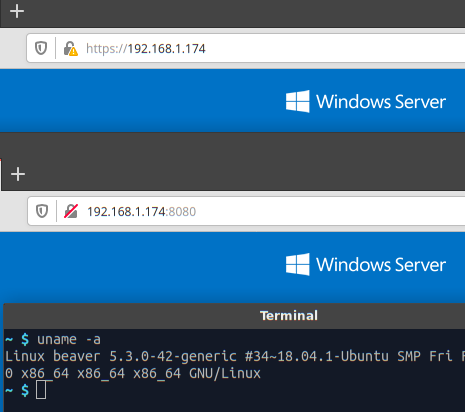
\includegraphics[scale=0.7]{i.png}\\
  \caption{Acceso al mismo site tanto desde el puerto 8080 (HTTP) como desde el 443 (HTTPS) a través de Linux}
  \label{fig:http_https}
\end{figure}

\pagebreak

\item %j
Para aplicar el modo ``Constrained Language'' a Powershell a nivel de sistema podemos establecer la variable \_\_PSLockDownPolicy a 4. En PowerShell escribimos \cite{powershell3}:
\begin{lstlisting}[language=bash]
[Environment]::SetEnvironmentVariable('__PSLockdownPolicy', '4', 'Machine')
\end{lstlisting}
Si queremos hacer un bypass de este modo, podemos bypasear primero la variable de entorno \cite{bypass}:
\begin{lstlisting}[language=bash]
Set-ItemProperty 'hklm:\SYSTEM\CurrentControlSet\Control\Session Manager\Environment' -name "__PSLockdownPolicy" -Value 8
\end{lstlisting}

y ejecutar una nueva instancia de PowerShell:
\begin{lstlisting}[language=bash]
Start-Process -File PowerShell.exe
\end{lstlisting}
\begin{lstlisting}[language=bash]
PS C:\Users\Administrator> $ExecutionContext.SessionState.LanguageMode
FullLanguage
\end{lstlisting}
AMSI es el acrónimo de \textit{Antimalware Scan Interface} y se trata de un interface que permite a las aplicaciones y servicios integrarse con cualquier producto antimalware existente en la máquina. Ofrece protección antimalware a los usuarios finales y a sus datos \cite{amsi}.
\begin{figure}[h!]
  \centering
  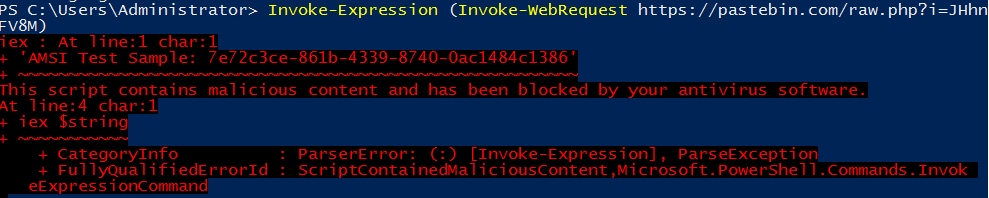
\includegraphics[scale=0.4]{j.png}\\
  \caption{AMSI habilitado en Powershell \cite{amsi2}}
  \label{fig:amsi}
\end{figure}
\pagebreak
\item %k
\begin{itemize}
\item nmap con la opción -sn es el modo \textit{host discovery}, escaneo con ping. \cite{manual}
\begin{figure}[h!]
  \centering
  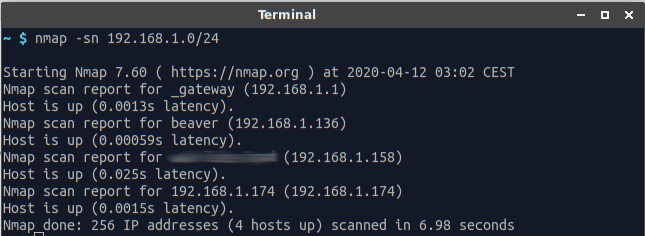
\includegraphics[scale=0.4]{k1.png}\\
  \caption{Listado de hosts en la red}
  \label{fig:nmap1}
\end{figure}

\item nmap con la opción -PI manda peticiones echo del protocolo ICMP.
\begin{figure}[h!]
  \centering
  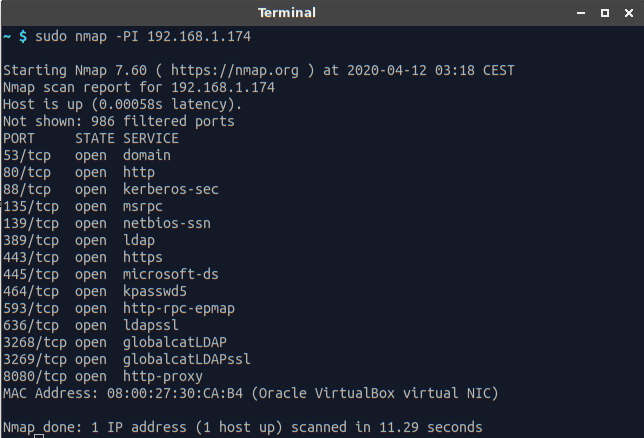
\includegraphics[scale=0.4]{k2.png}\\
  \caption{Escaneo de la red de Windows}
  \label{fig:nmap2}
\end{figure}

\item nmap con la opción -sS efectúa un escaneo TCP SYN o \textit{Stealth Scan}.
\begin{figure}[h!]
  \centering
  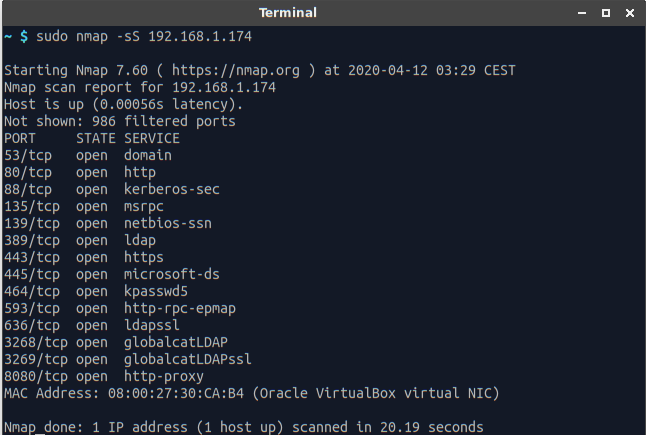
\includegraphics[scale=0.4]{k3.png}\\
  \caption{Escaneo SYN TCP de la red de Windows}
  \label{fig:nmap3}
\end{figure}
\pagebreak
\item nmap con la opción -sT efectúa un escaneo TCP Connect.
\begin{figure}[h!]
  \centering
  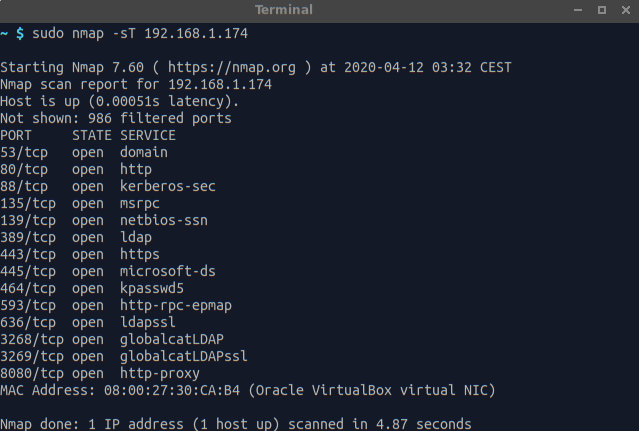
\includegraphics[scale=0.4]{k4.png}\\
  \caption{Escaneo TCP connect de la red de Windows}
  \label{fig:nmap4}
\end{figure}

\item nmap con la opción -sU efectúa un escaneo UDP.
\begin{figure}[h!]
  \centering
  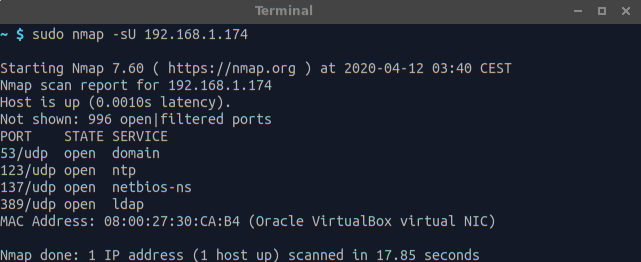
\includegraphics[scale=0.4]{k5.png}\\
  \caption{Escaneo UDP de la red de Windows}
  \label{fig:nmap5}
\end{figure}

\item nmap con la opción -O activa la detección del sistema operativo.
\begin{figure}[h!]
  \centering
  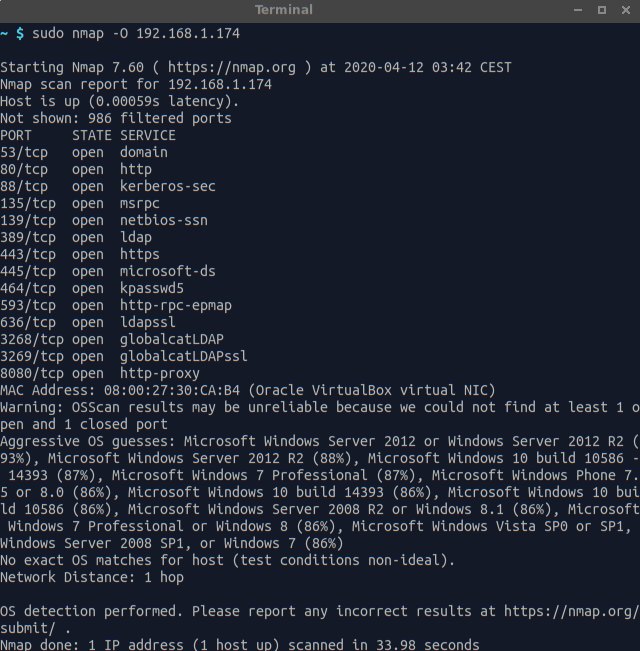
\includegraphics[scale=0.4]{k6.png}\\
  \caption{Escaneo para determinar el sistema operativo}
  \label{fig:nmap6}
\end{figure}
\pagebreak
\item nmap con la opción -sV nos da la versión de los servicios que se están ejecutando en los puertos.
\begin{figure}[h!]
  \centering
  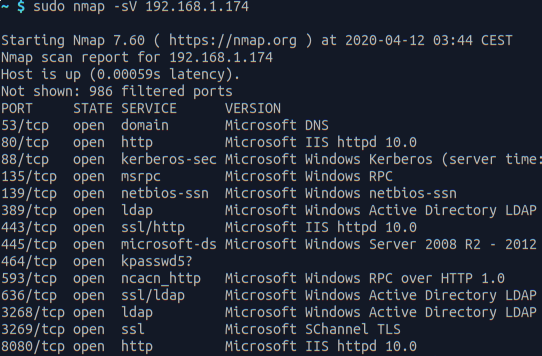
\includegraphics[scale=0.4]{k7.png}\\
  \caption{Escaneo para determinar las versiones de los servicios que están en marcha}
  \label{fig:nmap7}
\end{figure}

\end{itemize}

\end{enumerate}

\pagebreak
\begin{thebibliography}{9}

\bibitem{nginx}
  Techrepublic,\\
  \href{https://www.techrepublic.com/article/how-to-enable-ssl-on-nginx/}{How to enable SSL on NGINX}
  
  \bibitem{update-rc}
	solusan.com,\\
	\href{https://www.solusan.com/como-va-update-rcd-niveles-de-ejecucion-en-debian.html}{Cómo va update-rc.d ? (editor de niveles de ejecución en Debian)}
	
\bibitem{ping}
  Server Healers,\\
  \href{https://serverhealers.com/blog/disable-ping-response-icmp-echo-linux/}{How to Disable Ping Response ( ICMP echo ) in Linux}
  
\bibitem{boot}
	Ask Ubuntu,\\
	\href{https://askubuntu.com/questions/92556/how-do-i-boot-into-a-root-shell}{How do I boot into a root shell?}

\bibitem{grub}
	geekland,\\
	\href{https://geekland.eu/proteger-el-grub-con-contrasena/}{Proteger el grub con contraseña}

\bibitem{SCT}
Microsoft Security Compliance Toolkit 1.0,\\
	\href{https://docs.microsoft.com/en-us/windows/security/threat-protection/windows-security-configuration-framework/security-compliance-toolkit-10}{What is the Security Compliance Toolkit (SCT)?}
	
\bibitem{gpo_backup}
  Active Directory 360,\\
  \href{https://www.windows-active-directory.com/active-directory-group-policy-backup.html}{Group Policy Backup}
  
\bibitem{powershell}
  PowerShell Constrained Language Mode,\\
  \href{https://devblogs.microsoft.com/powershell/powershell-constrained-language-mode/}{What is PowerShell Constrained Language?}
 
\bibitem{powershell3}
	IT for Dummies,\\
	\href{https://itfordummies.net/2015/06/01/powershell-constrained-mode/}{PowerShell Constrained mode}

\bibitem{bypass}
   GitHub - Metoraf007,\\
	\href{https://github.com/Metoraf007/Public_PowerShell/blob/master/Bypass_ConstrainedLang.ps1}{PowerShell - Bypass Constrained Language Mode}
	
\bibitem{amsi}
   Windows Dev Center,\\
	\href{https://docs.microsoft.com/en-us/windows/win32/amsi/antimalware-scan-interface-portal}{Antimalware Scan Interface (AMSI)}
	
\bibitem{amsi2}
   Windows Dev Center,\\
	\href{https://docs.microsoft.com/en-us/windows/win32/amsi/how-amsi-helps}{How the Antimalware Scan Interface (AMSI) helps you defend against malware}

\bibitem{nmap-netstat}
	Stack Exchange - Superuser,\\	
	\href{https://superuser.com/questions/1065478/what-is-the-difference-between-nmap-and-netstat}{What is the difference between nmap and netstat?}

\bibitem{https-win}
	Sophos Community,\\
	\href{https://community.sophos.com/kb/en-us/132438}{How to Create a Self Signed SSL Certificate with Windows Server}

\bibitem{manual}
	nmap.org,\\
	\href{https://nmap.org/book/man.html}{Chapter 15. Nmap Reference Guide}
  
\end{thebibliography}

\end{document}